\documentclass[12pt, a4paper]{article}
\usepackage{../../../myconfig} % Gọi file cấu hình từ ngoài gốc vào

% ==========================================
% BẮT ĐẦU NỘI DUNG TÀI LIỆU
% ==========================================
\begin{document}

% Truyền 3 tham số: {Nhãn cam} {Chữ to chính giữa} {Chữ ở góc phải Header}
\titlebox{Chủ đề: Tích phân}{Ứng dung tích phân tính diện tích thể tính}{Nguyên hàm - Tích phân: Ứng dụng}

% --- CÂU 1 ---
\questionLinesManual{0}{1}{Diện tích hình phẳng giới hạn bởi đồ thị hàm số \( y = x^3 - 4x \), trục hoành và hai đường thẳng \( x = 0 \), \( x = 3 \) bằng:}{%
    \begin{tasks}(4)
        \task \( \displaystyle\int_{0}^{3} |x^3 - 4x| dx \)
        \task \( \displaystyle\pi \int_{0}^{3} |x^3 - 4x| dx \)
        \task \( \displaystyle\pi \int_{0}^{3} (x^3 - 4x)^2 dx \)
        \task \( \displaystyle\int_{0}^{3} (x^3 - 4x) dx \)
    \end{tasks}
}

% --- CÂU 2 ---
\questionLinesManual{0}{2}{Diện tích \( S \) của hình phẳng giới hạn bởi các đường \( y = 3x^2 \), \( y = -2 \), \( x = 0 \) và \( x = 1 \) được tính bởi công thức nào sau đây?}{%
    \begin{tasks}(4)
        \task \( \displaystyle\int_{0}^{1} (3x^2 + 2) dx \)
        \task \( \displaystyle\int_{0}^{1} |3x^2 - 2| dx \)
        \task \( \displaystyle\pi \int_{0}^{1} (3x^2 + 2)^2 dx \)
        \task \( \displaystyle\pi \int_{0}^{1} (3x^2 + 1)^2 dx \)
    \end{tasks}
}

% --- CÂU 3 ---
\questionLinesManual{0}{3}{Cho hình phẳng \( (H) \) giới hạn bởi đồ thị \( y = 2x - x^2 \) và trục hoành. Thể tích vật thể tròn xoay sinh ra khi cho \( (H) \) quay quanh trục hoành bằng}{%
    \begin{tasks}(4)
        \task \( \dfrac{16}{15} \)
        \task \( \dfrac{4}{3} \)
        \task \( \dfrac{16\pi}{15} \)
        \task \( \dfrac{4\pi}{3} \)
    \end{tasks}
}

% --- CÂU 4 ---
\questionLinesManual{0}{4}{Tính thể tích \( V \) của phần vật thể giới hạn bởi hai mặt phẳng \( x = 0, x = 1 \), có thiết diện bị cắt bởi mặt phẳng vuông góc với trục \( Ox \) tại điểm có hoành độ \( x(0 \leq x \leq 1) \) là một tam giác đều có cạnh bằng \( x \).}{%
    \begin{tasks}(4)
        \task \( V = \dfrac{12\pi}{5} \)
        \task \( V = \dfrac{12}{5} \)
        \task \( V = \dfrac{\sqrt{3}\pi}{12} \)
        \task \( V = \dfrac{\sqrt{3}}{12} \)
    \end{tasks}
}

% --- CÂU 5 ---
\questionLinesManual{0}{5}{Cho hình phẳng \( (H) \) giới hạn bởi các đường  
\( y = x^2 + 3, \, y = 0, \, x = 0, \, x = 2. \)  
Gọi \( V \) là thể tích khối tròn xoay được tạo thành khi quay \( (H) \) xuống quanh trục \( Ox \). Mệnh đề nào sau đây đúng?}{%
    \begin{tasks}(4)
        \task \( \displaystyle V = \pi \int_{0}^{2} (x^2 + 3) dx \)
        \task \( \displaystyle V = \int_{0}^{2} (x^2 + 3) dx \)
        \task \( \displaystyle V = \pi \int_{0}^{2} (x^2 + 3)^2 dx \)
        \task \( \displaystyle V = \int_{0}^{2} (x^2 + 3)^2 dx \)
    \end{tasks}
}

% --- CÂU 6 ---
\questionLinesManual{0}{6}{Diện tích của hình phẳng được tô màu trong hình bên dưới được tính theo công thức nào?

\begin{center}
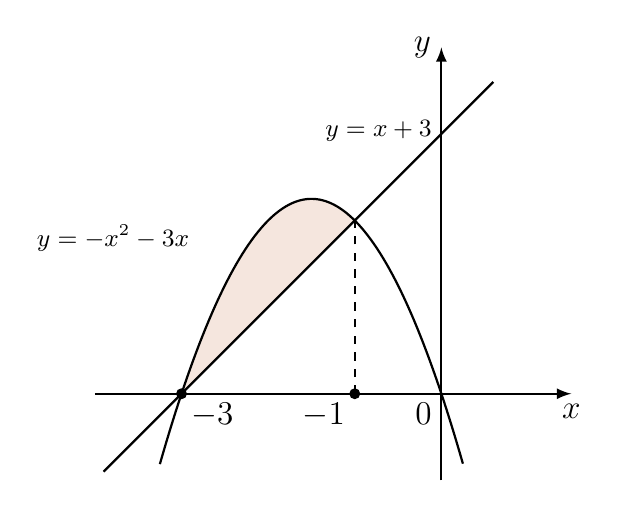
\begin{tikzpicture}[>=latex, scale=1.1]
    % Định nghĩa màu tô cho miền giới hạn (màu nâu/cam nhạt)
    \definecolor{fillcolor}{RGB}{245, 230, 222}
    \definecolor{brownline}{RGB}{139, 69, 19}

    % 1. Tô màu miền giới hạn giữa Parabola và Đường thẳng
    \fill[fillcolor] 
        plot[domain=-3:-1, samples=100] (\x, {-\x*\x - 3*\x}) -- 
        plot[domain=-1:-3, samples=100] (\x, {\x + 3}) -- cycle;

    % 2. Trục tọa độ
    \draw[->, thick] (-4.0,0) -- (1.5,0) node[below] {\large $x$};
    \draw[->, thick] (0,-1) -- (0,4) node[left] {\large $y$};

    % 3. Đồ thị các hàm số
    % Parabola y = -x^2 - 3x (Phần trong miền tô màu làm đậm màu nâu)
    \draw[thick, samples=100, domain=-3.25:0.25] 
        plot (\x, {-\x*\x - 3*\x});
    \node[left] at (-2.8, 1.8) {\small $y = -x^2 - 3x$};

    % Đường thẳng y = x + 3
    \draw[thick, domain=-3.9:0.6] 
        plot (\x, {\x + 3});
    
    \node[above left] at (0, 2.8) {\small $y = x + 3$};

    % 4. Đường gióng nét đứt và điểm giao
    \draw[dashed, thick] (-1,0) -- (-1,2);

    \fill (-3,0) circle (1.8pt) node[below right] {\large $-3$};
    \fill (-1,0) circle (1.8pt) node[below left] {\large $-1$};
    \node[below left] at (0,0) {\large $0$};
\end{tikzpicture}
\end{center}
}{%
    \begin{tasks}(4)
        \task \( \displaystyle\int_{-3}^{-1} (-x^2 - 4x - 3) dx \)
        \task \( \displaystyle\int_{-3}^{-1} (x^2 + 4x - 3) dx \)
        \task \( \displaystyle\int_{-3}^{-1} (-x^2 - 4x + 3) dx \)
        \task \( \displaystyle\int_{-3}^{-1} (x^2 + 4x + 3) dx \)
    \end{tasks}
}

% --- CÂU 7 ---
\questionLinesManual{0}{7}{Cho hình phẳng \( (H) \) giới hạn bởi các đường \( y = x^2 - 2x - 1 \), \( y = 2x - 4 \). Diện tích hình phẳng giới hạn bởi hình \( (H) \) bằng}{%
    \begin{tasks}(4)
        \task \( \dfrac{2}{3} \)
        \task \( \dfrac{4}{3} \)
        \task \( \dfrac{8}{3} \)
        \task 4
    \end{tasks}
}

% --- CÂU 8 ---
\questionLinesManual{0}{8}{Cho hàm số \( y = f(x) \). Biết rằng phần hình phẳng giới hạn bởi \( S_1 \) và \( S_2 \) (xem hình vẽ dưới đây) có diện tích lần lượt bằng 7 và 2. Tích phân \(\displaystyle\int_{-1}^{4} f(x) dx\) bằng

\begin{center}
\begin{tikzpicture}[>=latex, scale=0.9]
    % Thư viện cần dùng: \usetikzlibrary{patterns}

    % Định nghĩa màu sắc cho hai miền
    \definecolor{cyanfill}{RGB}{135, 206, 235}  % Màu xanh lam nhạt cho S1
    \definecolor{orangefill}{RGB}{245, 200, 140} % Màu cam nhạt cho S2

    % 1. Tô nền và gạch chéo cho miền S1 (từ x = -1 đến x = 2)
    \fill[cyanfill] 
        plot[domain=-1:2, samples=100] (\x, {0.25*(\x+1)*(\x-2)*(\x-4)}) -- 
        (2,0) -- (-1,0) -- cycle;
    \fill[pattern=north east lines, pattern color=black!60] 
        plot[domain=-1:2, samples=100] (\x, {0.25*(\x+1)*(\x-2)*(\x-4)}) -- 
        (2,0) -- (-1,0) -- cycle;

    % 2. Tô nền và gạch chéo cho miền S2 (từ x = 2 đến x = 4)
    \fill[orangefill] 
        plot[domain=2:4, samples=100] (\x, {0.25*(\x+1)*(\x-2)*(\x-4)}) -- 
        (4,0) -- (2,0) -- cycle;
    \fill[pattern=north east lines, pattern color=black!60] 
        plot[domain=2:4, samples=100] (\x, {0.25*(\x+1)*(\x-2)*(\x-4)}) -- 
        (4,0) -- (2,0) -- cycle;

    % 3. Trục tọa độ
    \draw[->, thick] (-1.8,0) -- (4.8,0) node[below] {\large $x$};
    \draw[->, thick] (0,-1.5) -- (0,2.8) node[left] {\large $y$};
    \node[below left] at (0,0) {\large $O$};

    % 4. Đồ thị hàm số y = f(x)
    \draw[very thick, samples=100, domain=-1.35:4.3] 
        plot (\x, {0.25*(\x+1)*(\x-2)*(\x-4)}) 
        node[above] {\large $y = f(x)$};

    % 5. Nhãn miền S1, S2 và các mốc tọa độ
    \node at (0.5, 0.8) {\Large $S_1$};
    \node at (3.0, -0.6) {\Large $S_2$};

    \node[above left] at (-1,0) {\large $-1$};
    \node[below left] at (2,0) {\large $2$};
    \node[below right] at (4,0) {\large $4$};
\end{tikzpicture}
\end{center}
}{%
    \begin{tasks}(4)
        \task 9
        \task -5
        \task -9
        \task 5
    \end{tasks}
}

% --- CÂU 9 ---
\questionLinesManual{0}{9}{Cho hàm số \( y = f(x) \) có đồ thị như Hình. Gọi \( S \) là phần diện tích hình phẳng được tô màu. Phát biểu nào sau đây là đúng?

\begin{center}
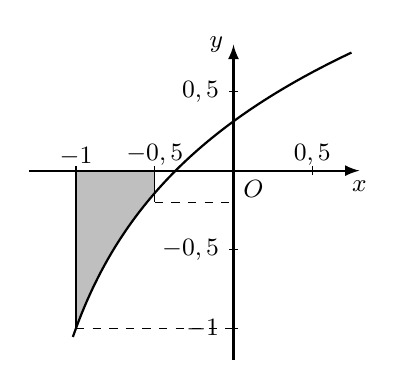
\begin{tikzpicture}[>=latex, scale=2.0]
    % 1. Tô màu xám miền giới hạn (từ x = -1 đến x = -0.5)
    % Hàm số phác họa: y = ln(x + 1.368)
    \fill[gray!50] 
        plot[domain=-1:-0.5, samples=100] (\x, {ln(\x + 1.367879)}) -- 
        (-0.5,0) -- (-1,0) -- cycle;

    % 2. Trục tọa độ
    \draw[->, thick] (-1.3,0) -- (0.8,0) node[below] {\small $x$};
    \draw[->, thick] (0,-1.2) -- (0,0.8) node[left] {\small $y$};
    \node[below right] at (0,0) {\small $O$};

    % 3. Đánh dấu các mốc tọa độ
    % Trục Ox
    \draw (-1,0.03) -- (-1,-0.03) node[above] {\small $-1$};
    \draw (-0.5,0.03) -- (-0.5,-0.03) node[above] {\small $-0,5$};
    \draw (0.5,0.03) -- (0.5,-0.03) node[above] {\small $0,5$};

    % Trục Oy
    \draw (0.03,-1) -- (-0.03,-1) node[left] {\small $-1$};
    \draw (0.03,-0.5) -- (-0.03,-0.5) node[left] {\small $-0,5$};
    \draw (0.03,0.5) -- (-0.03,0.5) node[left] {\small $0,5$};

    % 4. Đồ thị hàm số
    \draw[thick, samples=100, domain=-1.02:0.75] 
        plot (\x, {ln(\x + 1.367879)});

    % 5. Các đường gióng nét đứt và nét liền
    \draw[dashed] (-1,-1) -- (0,-1);
    \draw[dashed] (-0.5,-0.2) -- (0,-0.2);
    
    % Đường đứng ranh giới tại x = -1 và x = -0.5
    \draw (-1,0) -- (-1,-1);
    \draw (-0.5,0) -- (-0.5,-0.2);
\end{tikzpicture}
\end{center}
}{%
    \begin{tasks}(4)
        \task \( S = \displaystyle\int_{-1}^{-0,5} f(x) dx \)
        \task \( S = -\displaystyle\int_{-1}^{-0,5} f(x) dx \)
        \task \( S = -\left| \displaystyle\int_{-1}^{-0,5} f(x) dx \right| \)
        \task \( S = -\displaystyle\int_{-1}^{0,5} f(x) dx \)
    \end{tasks}
}

% --- CÂU 10 ---
\questionLinesManual{0}{10}{Tính diện tích hình phẳng giới hạn bởi đồ thị hàm số \( y = e^x \), trục hoành và hai đường thẳng  
\( x = 0 \) và \( x = 3 \).}{%
    \begin{tasks}(4)
        \task \( e^3 \)
        \task \( e^3 - 1 \)
        \task \( e^2 - 1 \)
        \task \( e(e^2 - 1) \)
    \end{tasks}
}

\end{document}
